%\documentclass[ignorenonframetext, professionalfonts, hyperref={pdftex, unicode}]{beamer}
\documentclass[pdftex,12pt,a4paper]{report}
\usepackage{beamerarticle}

\usetheme{Copenhagen}
\usecolortheme{wolverine}

%Packages to be included
\usepackage{graphicx}

\usepackage[T2A,T1]{fontenc}
\usepackage[utf8]{inputenc}
\usepackage[russian]{babel}

%%\usepackage[orientation=landscape, size=custom, width=16, height=9.75, scale=0.5]{beamerposter}

\usepackage{textcomp}

%\usepackage{beamerthemesplit}

\usepackage{ulem}

\usepackage{verbatim}

\usepackage{ucs}

\usepackage{url}

\usepackage{listings}
\lstloadlanguages{bash}

\lstset{escapechar=`,
	extendedchars=false,
	language=sh,
	frame=single,
	tabsize=2, 
	columns=fullflexible, 
%	basicstyle=\scriptsize,
	keywordstyle=\color{blue}, 
	commentstyle=\itshape\color{brown},
%	identifierstyle=\ttfamily, 
	stringstyle=\mdseries\color{green}, 
	showstringspaces=false, 
	numbers=left, 
	numberstyle=\tiny, 
	breaklines=true, 
	inputencoding=utf8,
	keepspaces=true,
	morekeywords={u\_short, u\_char, u\_long, in\_addr}
	}

\definecolor{darkgreen}{cmyk}{0.7, 0, 1, 0.5}

\lstdefinelanguage{diff}
{
    morekeywords={+, -},
    sensitive=false,
    morecomment=[l]{//},
    morecomment=[s]{/*}{*/},
    morecomment=[l][\color{darkgreen}]{+},
    morecomment=[l][\color{red}]{-},
    morestring=[b]",
}

\author[Epam]{{\bf Epam}\\Low Level Programming Department}

%\institution[EPAM]{EPAM}
\logo{\includegraphics[width=1cm]{logo.png}}

\usepackage[unicode=true]{hyperref}
\hypersetup{
    pdfkeywords={Linux},
    bookmarksnumbered=true,
    bookmarksopen=true,
    bookmarksopenlevel=1,
    colorlinks=true,
    pdfstartview=Fit,
    pdfpagemode=UseOutlines,
    pdfpagelayout=TwoPageRight
}

\newcommand{\defaultuser}{cur\_user}

\title{Основы Linux}

\begin{document}
\maketitle

\tableofcontents

\part{Основы Linux}

\begin{frame}{Основы ОС Linux}

	\begin{block}{Вопрос}
	Почему Linux является самой популярной
	свободной операционной системой?
	\end{block}

	\pause

	\begin{block}{Ответ}
	\begin{itemize}
		\item \textcopyleft -- Copyleft
		\item ``Философия'' Unix
		\item Открытые стандарты
	\end{itemize}
	\end{block}

\end{frame}


%%%%%%%%%%%%%%%%%%%%%%%%%%%%%%%%%%%%%%%%%   
%%%%%%%%%% Content starts here %%%%%%%%%%
%%%%%%%%%%%%%%%%%%%%%%%%%%%%%%%%%%%%%%%%%

\section[Принципы]{Базовые принципы ОС Linux}

\subsection{GNU/Linux}

\mode<all>{\input{../../slides/intro/vocabulary}}

\subsection{Лицензии}

\mode<all>{\begin{frame}{Авторское право и лицензии}

	\begin{block}{Авторское право}
		 Возникает по факту создания ПО 

		\begin{itemize}
			\item Неимущественные права
			\item Имущественные права
		\end{itemize}
	\end{block}

	\pause

	\begin{block}{Лицензии}
		Лицензия -- средство передать какие-либо права на продукт либо его часть.

		Необходима для защиты авторских прав. 
		Средство для возможности законно пресечь несанкционирование копирование,  использование или распространение ПО. 
	\end{block}
\end{frame}


\begin{frame}{Лицензии: открытые и свободные}
	\begin{block}{ Р.Столлман: 4 свободы}
		\begin{itemize}
			\item Свобода 0: Свобода запускать программу в любых целях.
			\item Свобода 1: Свобода изучения работы программы и адаптация её к вашим нуждам. 
				Доступ к исходным текстам является необходимым условием.
			\item Свобода 2: Свобода распространять копии,  так что вы можете помочь вашему товарищу.
			\item Свобода 3: Свобода улучшать программу и публиковать ваши улучшения,
				так что всё общество выиграет от этого.
				Доступ к исходным текстам является необходимым условием.
		\end{itemize}
	\end{block}
\end{frame}


\begin{frame}{Лицензии: permissive}
	\begin{columns}
	\column{0.3\textwidth}
		\center
\includegraphics[width=2cm,natwidth=144,natheight=144]{../../slides/intro/three-arrows@2x.png}

	\column{0.6\textwidth}

	\begin{itemize}
		\item BSD
		\item MIT
		\item Apache
	\end{itemize}
	\end{columns}

	\begin{block}{I want it simple and permissive.}
		\begin{itemize}
			\item практически не ограничивают свободу действий пользователей ПО и разработчиков, работающих с исходным кодом.
			\item По своему духу, распространение работы под пермиссивной лицензией схоже с помещением работы в общественное
				достояние, но не требует отказа от авторского права.
		\end{itemize}
	\end{block}

\end{frame}


\begin{frame}{\textcopyleft -- Copyleft}

	\begin{columns}
	\column{0.3\textwidth}
		\center
\includegraphics[width=2cm,natwidth=144,natheight=138]{../../slides/intro/circular@2x.png}

	\column{0.6\textwidth}

	\begin{itemize}
		\item GPL
		\item LGPL
		\item AGPL
	\end{itemize}
	\end{columns}


	\begin{block}{I care about sharing improvements.}
	
	Авторское лево -- концепция и практика использования законов авторского права для обеспечения 
	невозможности ограничить любому человеку право использовать,  изменять и распространять как 
	исходное произведение,  так и произведения,  производные от него.
	\end{block}


	При копилефте все производные произведения должны распространяться под той же лицензией,
	что и оригинальное произведение.

\end{frame}



}

\subsection{Принципы проектирования переносимых программ}

\mode<all>{\begin{frame}{Главные ориентиры}
	\begin{itemize}
		\item кроссплатформенная переносимость
		\item открытые стандарты
	\end{itemize}
\end{frame}

\begin{frame}{Немного цитат}
Дуг Макилрой, изобретатель каналов <<pipes>>, сформулировал несколько постулатов,применимых для разработки ПО:
\pause
	\begin{itemize}
		\item пишите программы,  которые выполняют одну функцию и делают это хорошо;
			\pause
		\item пишите программы,  которые будут работать вместе;
			\pause
		\item пишите программы,  поддерживающие текстовые потоки,  поскольку они являются универсальным интерфейсом.
	\end{itemize}

\end{frame}


\begin{frame}{"Философия" UNIX}
	это {\bfseries не} философия,  а общие рекомендации по проектированию ПО,  накопленные сообществом программистов на опыте десятилетий разработок программ,  которые взаимодействуют друг с другом.
\end{frame}

\begin{frame}{1. Правило модульности}
	\begin{block}{Следует писать простые части,  связанные ясными интерфейсами.}
Единственным способом создания сложной программы,  не обреченной заранее на провал,  является сдерживание ее глобальной сложности.
	\end{block}
Т.е. построение программы из простых частей, соединенных четко определенными интерфейсами, 
так что большинство проблем являются локальными, 
и тогда можно рассчитывать на обновление одной из частей без разрушения целого.
\end{frame}

\begin{frame}{Размер кода и ошибки}
	\begin{center}
		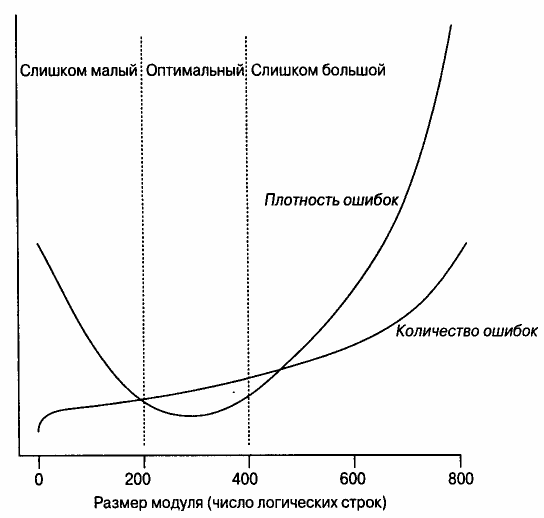
\includegraphics[width=200px]{../../slides/intro/errors_density-graph.png}
	\end{center}
\end{frame}

\begin{frame}{2. Правило ясности}
	\begin{block}{Ясность -- лучше чем мастерство.}
		Последующее обслуживание программы -- важная и дорогостоящая часть жизненного цикла программы.
	\end{block}
	\pause
Писать программы необходимо так,  как если бы вы знали,  что последующей поддержкой будет заниматься неуравновешенный псих с топором,  знающий ваш домашний адрес!
\end{frame}

\begin{frame}{3. Правило композиции}
	\begin{block}{Следует разрабатывать программы,  которые будут взаимодействовать с другими программами.}
		Если разрабатываемые программы не способны взаимодействовать друг с другом,  то очень трудно избежать создания сложных монолитных  программ.
	\end{block}
	Методы взаимодействия могут быть сильными и слабыми -- по возможности рекомендуется использовать слабые методы и текстовые форматы передачи данных.
\end{frame}

\begin{frame}{4. Правило разделения}
	\begin{block}{Следует отделять политику от механизма и интерфейсы от основных модулей (engine).}
		Примеры политики и механизма:\\
		вид GUI и операции отрисовки, клиент (front-end) -- сервер (back-end), сценарии и библиотеки и др.
	\end{block}
	При жесткой связи политики и механизма:
	\begin{itemize}
		\item политика становится негибкой и усложняется ее изменение;
		\item изменение политики имеет строгую тенденцию к дестабилизации механизмов.
	\end{itemize}
\end{frame}

\begin{frame}{5. Правило простоты}
	\begin{block}{Необходимо проектировать простые программы и <<добавлять сложность>> только там,  где это необходимо.}
	\end{block}
	Основные причины добавления сложности:
	\begin{itemize}
		\item человеческий фактор (часто -- желание <<выпендриться>>);
		\item проектные требования,  продиктованные текущей модой,  маркетингом или «левой пяткой заказчика»;
	\end{itemize}
\end{frame}

\begin{frame}{6. Правило расчетливости}
	\begin{block}{Пишите большие программы,  только если после демонстрации становится ясно,  что ничего другого не остается.}
		Под <<большими программами>> здесь понимаются программы с большим объемом кода и значительной внутренней сложностью.
	\end{block}
\end{frame}

\begin{frame}{7. Правило прозрачности}
	\begin{block}{Для того,  чтобы упростить проверку и отладку программы,  ее конструкция должна быть обозримой.}
		Программа {\itshape прозрачна}, если при ее минимальном изучении можно понять, что она делает и как.\\
		Программа {\itshape воспринимаема},  когда она имеет средства для мониторинга и отображения внутреннего состояния.
	\end{block}
	Необходимо использовать достаточно простые форматы входных и выходных данных.\\
	Интерфейс должен быть приспособлен для использования в отладочных сценариях.
\end{frame}

\begin{frame}{8. Правило устойчивости}
	\begin{block}{Устойчивость -- следствие	прозрачности и простоты.}
		Программа является {\itshape устойчивой},  когда она выполняет свои функции в неожиданных условиях,  которые выходят за рамки предположений разработчика,  как и в нормальных условиях.\\
		Программа является {\itshape простой},  если происходящее в ней не представляется сложным для восприятия человеком.
	\end{block}
	Один из способов организации -- модульность(простые блоки,  ясные интерфейсы)\\
	Следует избегать частных случаев!
\end{frame}

\begin{frame}{Пример неусточивого ПО}
	\begin{center}
		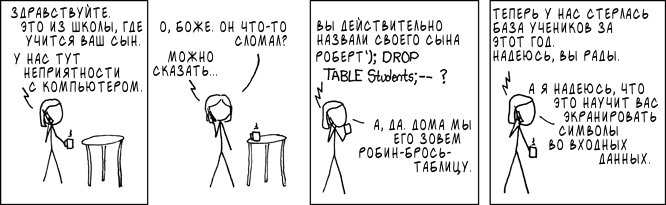
\includegraphics[width=1\textwidth]{../../slides/intro/exploits_of_a_mom_rus.png}
	\end{center}
\end{frame}


\begin{frame}[fragile]{Пример <<простой>> программы}
	\begin{center}
		\begin{verbatim}
+++++++++++++++++++++++++++++++++++++++++++++
+++++++++++++++++++++++++++.+++++++++++++++++
++++++++++++.+++++++..+++.-------------------
---------------------------------------------
---------------.+++++++++++++++++++++++++++++
++++++++++++++++++++++++++.++++++++++++++++++
++++++.+++.------.--------.------------------
---------------------------------------------
----.-----------------------.
		\end{verbatim}
	\end{center}
\end{frame}

\begin{frame}{9. Правило представления}
	\begin{block}{Знания следует оставлять в данных,  чтобы логика программы могла быть примитивной и устойчивой.}
		Даже простую логику бывает сложно проверить,  но даже сложные структуры данных являются довольно простыми для моделирования и анализа (например диаграмма 50 узлов дерева и блок-схема 50 строк кода)
	\end{block}
	Если можно выбирать между усложнением структуры данных и усложнением кода,  то лучше выбирать первое.\\
	Примеры: ascii,  генератор html-таблицы.
\end{frame}

\begin{frame}{10. Правило наименьшего удивления}
	\begin{block}{При проектировании интерфейсов всегда следует использовать наименее неожиданные элементы.}
		Необходимо учитывать характер предполагаемой аудитории и традиции платформы.
	\end{block}
	Оборотная сторона: следует избегать создания внешне похожих вещей,  слегка отличающихся в действительности,  поскольку {\itshape кажущаяся привычность порождает ложные ожидания}.
\end{frame}

\begin{frame}{11. Правило тишины}
	\begin{block}{Если программе нечего сказать,  то пусть лучше молчит.}
		Внимание и сосредоточенность пользователя -- ценный и ограниченный ресурс,  который требуется только в случае необходимости.
	\end{block}
	Важная информация не должна смешиваться с подробными сведениями о работе программы.
\end{frame}

\begin{frame}{12. Правило восстановления}
	\begin{block}{Когда программа завершается аварийно,  это должно происходить явно (шумно) и по возможности быстро.}
		Если программа не способна справиться с ошибкой,  то необходимо завершить ее работу так,  чтобы максимально упростить диагностику.
	\end{block}
	Для сетевых служб следует следовать рекомендации Постела:\\
	<<{\itshape Будьте либеральны к тому,  что принимаете,  и консервативны к тому,  что отправляете}>>
\end{frame}

\begin{frame}{13. Правило экономии}
	\begin{block}{Время программиста дорого -- поэтому задача экономии его времени более приоритетна,  по сравнению с экономией машинного времени.}
		Компьютер железный -- ему не скучно (с) программистская мудрость
	\end{block}
	Использование высокоуровневых языков и <<обучение>> машины выполнять больше низкоуровневой работы по программированию,  что приводит к правилу 14.
\end{frame}

\begin{frame}{14. Правило генерации}
	\begin{block}{Избегайте кодирования вручную; если есть возможность -- пишите программы для создания программ.}
		Использование генераторов кода оправданно,  когда они могут повысить уровень абстракции,  
		т.е. когда язык спецификации для генератора проще,  чем сгенерированный код,  
		и код впоследствии не потребует ручной доработки.
	\end{block}
	Примеры: грамматические и лексические анализаторы,  генераторы make-файлов,  построители GUI-интерфейсов.
\end{frame}

\begin{frame}{15. Правило оптимизации}
	\begin{block}{Сначала -- опытный образец,  потом -- оптимизирование.}
		Добейтесь стабильной работы,  только потом оптимизируйте.
	\end{block}
	\begin{block}{Керниган и Плоджер:}
		90\% актуальной и реальной функциональности лучше,  чем 100\% функциональности перспективной и сомнительной
	\end{block}
	\begin{block}{Кнут:}
		преждевременная оптимизация -- корень всех зол
	\end{block}
	\begin{block}{Кент Бек (экстремальное программирование):}
		заставьте программу работать,  заставьте работать ее верно,  а затем сделайте ее быстрой
	\end{block}
\end{frame}

\begin{frame}{16. Правило разнообразия}
	\begin{block}{Не следует доверять утверждениям о <<единственно правильном пути>>.}
		Никто не обладает умом,  достаточым для оптимизации всего или для предвидения всех возможных вариантов использования создаваемой программы.
	\end{block}
\end{frame}

\begin{frame}{17. Правило расширяемости}
	\begin{block}{Разрабатывайте для будущего. Оно наступит быстрее,  чем вы думаете.}
		При проектировании протоколов или форматов файлов следует делать их самоописательными,  для того,  чтобы их можно было расширить.
	\end{block}
	{\itshape Всегда},  следует либо включать номер версии,  либо составлять формат из самодостаточных,  
	самоописательных команд так,  чтобы можно было легко добавить новые директивы,  
	а старые удалить, <<не сбивая с толку>> код чтения формата.
\end{frame}

\begin{frame}{Все правила сразу}
	\begin{center}
	{\Huge\bfseries K.I.S.S.}

	Keep It Simple,  Stupid!
	\end{center}
\end{frame}


}

\section{Дистрибутивы ОС Linux}

\mode<all>{\begin{frame}{Дистрибутив ОС GNU/Linux}
	\begin{block}{ Определение}
		\only<1>{\center{\bf{?}}}
		\pause
		\only<2->{Набор программного обеспечения на базе ядра Linux, распространяющийся как единое целое.}
	\end{block}
\end{frame}


\begin{frame}{Задачи дистрибутива}
	\begin{itemize}
		\item Предоставление комплекта ПО (ядро + утилиты)
		\item Средства установки и настройки
		\item Средства обновления
	\end{itemize}
\end{frame}

\begin{frame}{Различия между дистрибутивами}

	\only<1>{\Large\center{\bf{?}}}
	\pause
	\only<2->{\Large\center{\bf{Цели!!!}}}

	\bigskip
	\normalsize

	\pause

	\begin{itemize}
		\begin{columns}
		\column{0.4\textwidth}
			\item Инсталлятор
			\item Первичные настройки
			\item Средства управления
			\item Набор ПО
		\column{0.4\textwidth}
			\item Менеджер пакетов
			\item Формат распространения ПО
			\item Пути к файлам
			\item Система сборки ПО
		\end{columns}
	\end{itemize}
\end{frame}

\begin{frame}{Дистрибутивы}
	\begin{itemize}
		\begin{columns}
		\column{0.3\textwidth}
			\item RedHat
			\item Fedora Core
			\item CentOS
			\item Scientific Linux
			\item Oracle Unbreakable Linux
		\column{0.3\textwidth}
			\item Slackware 
			\item Gentoo
			\item Arch
			\item OpenSUSE
			\item ALT Linux 
		\column{0.3\textwidth}
			\item Debian
			\item Ubuntu
			\item Mint
			\item Knoppix
			\item BackTrack
		\end{columns}
	\end{itemize}
\end{frame}
}

\section{Процесс загрузки ОС Linux}

\subsection{Этапы загрузки}

\mode<all>{\begin{frame}{Процесс загрузки GNU/Linux}
	\small
	\begin{enumerate}
		\item BIOS
		\item MBR
			\pause
		\item Загрузка загрузчика
		\begin{itemize}
		\scriptsize
			\item Stage 1 -- Первичный загрузчик
			\item Stage 1,5 -- Загрузка ядра загрузчика и драйвера ФС
			\item Stage 2 -- Чтение конфигурации
		\end{itemize}
			\pause

		\item Загрузка ядра в память
		\item Загрузка initrd в память
			\pause
		\item Передача управления ядру
		\begin{itemize}
		\scriptsize
			\item Распаковка
			\item Инициализация
		\end{itemize}

		\item Монтирование initrd
		\item Запуск программы инициализации в initrd
			\pause
		\item Нахождение и монтирование корневого раздела
			\pause
		\item Запуск программы init
		\begin{itemize}
		\scriptsize
			\item Монтирование оставшихся разделов ФС
			\item Инициализация оборудования
			\item Запуск демонов
		\end{itemize}

	\end{enumerate}
\end{frame}


\begin{frame}{Наиболее распространенные загрузчики}
	\begin{itemize}
		\item GRUB
		\item LILO
		\item syslinux (isolinux, pxelinux)
		\item u-boot
	\end{itemize}
\end{frame}
}

\subsection{Ядро Linux}

\mode<all>{\begin{frame}{Задачи ядра Linux}
	\begin{itemize}
		\item Инициализация системы
		\item Управление процессами и потоками
		\item Управление памятью
		\item Управление файлами
		\item IPC
		\item Разграничение доступа
		\item Сетевые возможности
		\item Интерфейс доступа к возможностям ядра
	\end{itemize}
\end{frame}


\begin{frame}{Ядро}

	Ядро ОС Linux является модульным. 

	\begin{block}{Модули}
		\begin{itemize}
			\item В виде отдельных файлов
			\item "Вкомпилированные" в ядро
		\end{itemize}
	\end{block}

	\bigskip

	Список загруженных модулей: {\tt /proc/modules}
\end{frame}


\begin{frame}{Параметры ядра}
	
	Полный список: {\tt Documentation/kernel-parameters.txt}

	\begin{block}{Некоторые часто применяемые параметры}
		\begin{itemize}
			\begin{columns}
			\column{0.3\textwidth}
				\item console=ttyS0,9600
				\item debug
				\item init=/sbin/init
				\item loglevel=[0-7]
				\item maxcpus=[num]
			\column{0.3\textwidth}
				\item mem=nn[KMG]
				\item noacpi
				\item noapic
				\item panic=nn (sec)
				\item resume=/dev/sda2
			\column{0.3\textwidth}
				\item ro
				\item rw
				\item root=/dev/sda1
				\item rootdelay=nn (sec)
				\item rootwait
				\item vga=<num>|ask
			\end{columns}
		\end{itemize}
	\end{block}

	Модулям можно передавать параметры используя синтаксис: {\tt module.param=value}

	Параметры переданные ядру во время загрузки: {\tt /proc/cmdline}
\end{frame}

\begin{frame}{Магия SysRq}

	{\tt CONFIG\_MAGIC\_SYSRQ=y}

	{\tt /proc/sysrq-trigger}

	\begin{block}{{\bf R}eboot {\bf E}ven {\bf I}f {\bf S}ystem {\bf U}tterly {\bf B}roken}
		{\bf Ctrl+Alt+SysRq+?}

		\begin{itemize}
			\item h -- вывести список сочетаний на консоль
			\item b -- перезагрузка
			\item o -- выключение
			\item e -- послать сигнал SIGTERM всем процессам кроме init
			\item i -- послать сигнал SIGKILL всем процессам кроме init
			\item s -- синхронизировать все ФС 
			\item u -- переподключить все ФС в режиме RO
		\end{itemize}
		
	\end{block}


\end{frame}
}

\subsection{Userspace}

\mode<all>{\input{../../slides/intro/initrd}}

\mode<all>{\begin{frame}{init}
	Менеджер управления работой системой и сервисами.
	
	\bigskip

	\center{\large PID = 1}

	\bigskip

	\begin{block}{Наиболее известные}
		\begin{itemize}
			\item SysVInit
			\item systemd
			\item upstart
		\end{itemize}
	\end{block}
\end{frame}

\begin{frame}{SysVInit}
	\begin{block}{Управление}
		\begin{itemize}
			\item kernel boot parameters: <N> -- runlevel
			\item утилита {\tt runlevel}
			\item утилита {\tt init}
		\end{itemize}
	\end{block}

	\scriptsize
	\begin{block}{Runlevel}
		\begin{table}
			\begin{tabular}{| c | l | }
			\hline
			Runlevel & Описание\\
			\hline
			0	& Выключить систему \\
			1,s,single & Однопользовательский режим \\
			2	& Многопользовательский режим без графики. Без сетевых сервисов.\\
			3	& Многопользовательский режим без графики. Полноценная сеть. \\
			4	& Определяется на хосте\\
			5	& Многопользовательский режим с графикой.\\
			6	& Перезагрузка\\
			emergency & Аварийная оболочка \\
			\hline
			\end{tabular}
		\end{table}
	\end{block}
\end{frame}

\begin{frame}{SysVInit: сервисы}
	\begin{block}{Управление}
		\begin{itemize}
			\item утилита {\tt service}
			\item утилита {\tt chkconfig}
		\end{itemize}
	\end{block}

	\begin{block}{Сервисы}
		\begin{itemize}
			\item {\tt /etc/rc.d/init.d}
			\item {\tt /etc/rc.d/rc.N}\footnote{N=runlevel}
		\end{itemize}
	\end{block}
\end{frame}

\begin{frame}{systemd}
	\begin{block}{Управление}
		\begin{itemize}
			\item kernel boot parameters\\
				{\tt systemd.unit=rescue.target} \\
			\item утилита {\tt systemctl} \\
				{\tt systemctl isolate multi-user.target} \\
				{\tt systemctl set-default single.target}
		\end{itemize}
	\end{block}

	\begin{block}{targets}
		\tiny
		\begin{table}
			\begin{tabular}{| c | l | l | }
			\hline
			Runlevel & Описание\\
			\hline
			0	& poweroff.target & Выключить систему \\
			1,s,single & rescue.target  & Однопользовательский режим \\
			2	& multi-user.target & Многопользовательский режим без графики. Без сетевых сервисов.\\
			3	& multi-user.target & Многопользовательский режим без графики. Полноценная сеть. \\
			4	& multi-user.target & Определяется на хосте\\
			5	& graphical.target & Многопользовательский режим с графикой.\\
			6	& reboot.target & Перезагрузка\\
			emergency & emergency.target & Аварийная оболочка \\
			\hline
			\end{tabular}
		\end{table}
	\end{block}
\end{frame}

\begin{frame}{systemd: сервисы}
	\begin{block}{Управление}
		\begin{itemize}
			\item утилита {\tt systemctl}
		\end{itemize}
	\end{block}

	\begin{block}{Сервисы}
		\begin{itemize}
			\item {\tt /lib/systemd/system/}
			\item {\tt /etc/systemd/system/}
		\end{itemize}
	\end{block}
\end{frame}
}

\subsection{Практика}

\mode<all>{\begin{frame}{Практическое задание}
	\begin{enumerate}
		\item Загрузить ОС по умолчанию
		\item Посмотреть используемые параметры ядра 
		\item Посмотреть список загруженных модулей
			\pause
		\item Переопределить init на sh
		\item SysRq. {\bf R}eboot {\bf E}ven {\bf I}f {\bf S}ystem {\bf U}tterly {\bf B}roken
			\pause
		\item Загрузить ядро с "урезанным" количеством памяти
		\item Отключить 1 или несколько процессоров
			\pause
		\item Посмотреть текущий runlevel
		\item Посмотреть список сервисов
	\end{enumerate}
\end{frame}
}




\part{Командная строка}

\section{Командная оболочка (shell)}

\mode<all>{\begin{frame}[fragile]{Определение(не совсем формальное)}
	\textbf{Shell} -- приложение, обеспечивающее выполнение других приложений и их взаимодействие, а также представляющая услуги командной строки. 
	\begin{center}
	 или
	\end{center}
	\textbf{Shell} -- приложение, обеспечивающее доступ к основным функциям ядра.

	\pause
	\vspace{0.5in}
	Пример shell из Windows-world -- cmd.exe
	\vspace{0.5in}

	Минимальный дистрибутив Linux -- ядро + shell 

\end{frame}

\begin{frame}[fragile]{Основные типы shell в Unix}
  \begin{itemize}
    \item Bourne shell совместимые
      \begin{itemize}
        \item \textbf{sh} исходная bourne shell (Steve Bourne, 1978)
        \item \textbf{ksh} Korn shell (David Korn, 1983)
        \item \textbf{ash} $[$BSD$]$ Almquist shell (Kenneth Almquist,1989)  
        \item \textbf{bash} $[$GPL$]$ Bourne-again shell (Brian Fox, 1989)
        \item \textbf{zsh} $[$BSD$]$ Z shell (Paul Falstad,1990)
        \item \textbf{/bin/sh} Указывает на POSIX-совместимую shell
      \end{itemize}
  \item C shell совместимые
      \begin{itemize}
        \item \textbf{csh}  Исходная С shell (Bill Joy, 1978)
        \item \textbf{tcsh} $[$BSD$]$ TENEX C shell (Ken Greer, 1981)
       \end{itemize}
  \end{itemize}
\end{frame}

\begin{frame}[fragile]{Маленькое упражнение}
\begin{lstlisting}[language=bash]
cat /etc/shells
ls -l <filename> # для каждого элемента /etc/shells
readlink -e <filename> 
\end{lstlisting}
\end{frame}


}

\section{Don't panic! Получение помощи}

\mode<all>{
\begin{frame}[fragile]{Как правильно задавать вопросы}
From FAQ How To Ask Questions The Smart Way
Before You Ask
  \begin{itemize}
	  \item Try to find an answer by reading the manual.
	  \item Try to find an answer by reading a FAQ.
	  \item Try to find an answer by searching the archives of the forum you plan to post to.
	  \item Try to find an answer by searching the Web.
	  \item Try to find an answer by inspection or experimentation.
	  \item Try to find an answer by asking a skilled friend.
	  \item If you're a programmer, try to find an answer by reading the source code.
    \end{itemize}
\end{frame}


\begin{frame}[fragile]{Источники получение помощи}
  \begin{itemize}
    \pause
    \item \textbf{man} - помощь по внешним командам
    \pause
    \item \textbf{help} - встроенная помощь по внутренним командам bash (также man bash)
    \pause
    \item \textbf{info} - расширенная помощь по некоторым командам (texinfo format)
     \begin{block}{Упражнение. Работа с командой info}
        \begin{itemize}
        \item   Попробовать {\tt info coreutils}
        \item   Справка по навигации -- нажать h
        \end{itemize}
	 \end{block}
		\begin{block}{Упражнение. Другие источники помощи.}
			\begin{lstlisting}
            help 
            help help
            man -h
            info --help
			\end{lstlisting}
		\end{block}
  \end{itemize}
\end{frame}

\begin{frame}[fragile]{Основное о man}
\begin{columns}
	\column{2.5in}
		\begin{itemize}
			\item Прочитайте {\tt man man} !
			\item apropos, аналог {\tt man -k <слово>}
            \item whatis, аналог {\tt man -f <слово>} 
			\item Разделы (sections)
				\begin{itemize}
					\item[1] Основная секция(юзерские программы)
					\item[2] Syscalls
					\item[3] С library
					\item[5] Конфигурационные файлы
					\item[8] Системные службы
				\end{itemize}
		\end{itemize}
	  \textbf{Замечание}

	  Обычно внутри страницы работает поиск с помощью '/'
	\pause 
	
	\column{1in}
		\begin{block}{Попробовать}
			\begin{lstlisting}
man -k intro or apropos
man -f intro or whatis
man 3 intro
man 1 intro
man -wa intro
			\end{lstlisting}
		\end{block}
	\end{columns}
\end{frame}


%\begin{frame}[fragile]{Чему научились}
%  \begin{itemize}
%  \item Как спрашивать у сообщества
%  \item Умеем использовать 3 источника получения информации man, info, help
%  \item Как перемещаться по страницам помощи info и man
%  \item Иcкать в системе помощи man и запрашивать из одного из 8-ми разделов 
%  \end{itemize}
%\end{frame}
}

\section{Навигация по файловой системе}

\mode<all>{\begin{frame}{Навигация по файловой системе}
      \begin{itemize}
		  \item {\tt ls} -- список файлов в (текущей по умолчанию) директории (man ls)
		  \item {\tt cd} -- смена текущей директории (help cd)
		  \item {\tt pwd} -- имя текущей директории (help pwd)
      \end{itemize}
\end{frame}

\begin{frame}[fragile]{Команды для работы с файлами}
	\begin{itemize}
		\begin{columns}
		\column{0.2\textwidth}
			\item touch
			\item ln
			\item mkdir
			\item mknod
			\item mkfifo
		\column{0.2\textwidth}
			\item cp
			\item mv
			\item install
			\item rm
			\item rmdir
			\item file
		\column{0.4\textwidth}
			\begin{block}{Упражнение}
				\begin{enumerate}
					\item Создать иерархию директорий
						\begin{lstlisting}
dir1/dir1.1/dir1.1.1
dir1/dir1.2/dir1.2.1
dir1/dir1.2/dir1.2.2
						\end{lstlisting}
					\item Внутри каждой создать файл
					\item Удалить все созданное
				\end{enumerate}
			\end{block}
		\end{columns}
	\end{itemize}
\end{frame}


}

\mode<all>{\begin{frame}{Файловая структура}
	
	{\center "Дерево внутри дома?" (c) Шрек}
		
	\begin{columns}
	\column{0.2\textwidth}
		\includegraphics[height=0.8\textheight]{../../slides/fs/01-lhs.png}
		
	\column{0.7\textwidth}
		\begin{itemize}
			\item Директории
			\item Обычные файлы
			\item Симлинки
			\item Хардлинки
			\item Файлы устройств
			\item FIFO
			\item сокеты
		\end{itemize}
	\end{columns}
\end{frame}
}

\section{Полезные инструменты bash}
\mode<all>{\begin{frame}{Важные аббревиатуры внутри командной строки}
  \begin{itemize}
    \item Для директорий
      \begin{itemize}
        \item {\tt $\sim$} Домашняя директория
        \item {\tt $\sim$<username>} Домашняя директория пользователя
        \item {\tt ..} Родительская директория
        \item {\tt .} Текущая директория
      \end{itemize}
      \pause  
    \item Wildcards
      \begin{itemize}
        \item {\tt *} Любой набор символов {\tt file*txt : file1.txt filefilefiletxt}
        \item {\tt $[$<список>$]$ } символ из заданного набора
        \item {\tt ?} любой один символ
      \end{itemize}

  \end{itemize}
\end{frame}       

\begin{frame}{Горячие клавиши}
  \begin{itemize}
    \item \textbf{Tab} -- дополнение текущей команды
      \pause
    \item История команд
      \begin{itemize}
        \item Клавиши курсора -- навигация по истории
        \item Ctrl-R -- поиск в истории по фрагменту
        \item Ctrl-O (после выполнения вставить следующую команду из истории)
        \item Команда {\tt history}
      \end{itemize}
    \item Навигация

  \end{itemize}
\end{frame}

\begin{frame}{Переменные окружения}
  \begin{itemize}
    \item {\tt HOME}
    \item {\tt PWD}
    \item {\tt LANG}
    \item {\tt LD\_LIBRARY\_PATH}
    \item {\tt SHELL}
    \item {\tt TERM}
    \item {\tt DISPLAY}
  \end{itemize}

  Контроль

  \begin{itemize}
    \item export {\tt export VAR=value}
    \item declare -x
    \item echo 
  \end{itemize}

  Переменные окружения наследуются при создании нового процесса
\end{frame}

%\begin{frame}{Настройки bash и кастомизация}
%  \begin{itemize}
%    \item Login shell
%      \begin{itemize}
%        \item {\tt /etc/profile}
%        \item {\tt $\sim$/.profile }
%      \end{itemize}
%    \item Обычная интерактивная shell
%      \begin{itemize}
%        \item {\tt /etc/bash.bashrc}
%        \item {\tt $\sim$/.bashrc}
%      \end{itemize}
%  \end{itemize}
%
%  Полезные команды
%  \begin{itemize}
%    \item {\tt alias}
%    \item {\tt export PATH=}
%    \item {\tt Определение функции}
%    \item {\tt shopts}
%  \end{itemize}
%
%\end{frame}


}

\part{Управление процессами и перенаправления}

\section{Процессы}
\mode<all>{\begin{frame}{Процессы в UNIX}
  \begin{itemize}
    \item Создание процессов
      \begin{itemize}
        \item fork
        \item exec
      \end{itemize}
    \item Атрибуты процесса
      \begin{itemize}
        \item pid 
        \item файловые дескрипторы
        \item environment
        \item Рабочая директория (cwd)
        \item прочее в директории {\tt /proc/<pid>}
      \end{itemize}
  \end{itemize}
\end{frame}

\begin{frame}{Управление процессами}
  \begin{itemize}
    \item kill (killall)
    \item top
    \item pstree
    \item Команды управления процессами в bash: 
      \begin{itemize}
        \item {\tt jobs}, {\tt fg, \tt bg}
        \item Ctrl-C -- оборвать выполнение процесса (SIGINT)
        \item Ctrl-Z -- остановить выполнение команды (SIGTSTP)
        \item Ctrl-D -- завершить ввод
      \end{itemize}
  \end{itemize}
\end{frame}


\begin{frame}{Упражнения}
  \begin{block}{Посмотреть вывод pstree}
    {\tt pstree}
  \end{block}
  \pause
  \begin{block}{Ctrl-C, Ctrl-Z}
    В графическом режиме запустить из терминала emacs

    Ctrl-Z

    jobs -l

    bg +
  \end{block}
  \pause
  \begin{block}{fork bomb}

    {\tt ulimit -u 200} 

    {\tt bomb()\{ (bomb; bomb) \& \} }

    top

    killall bash

  \end{block}
\end{frame}


\begin{frame}{Unix way}
  \begin{enumerate}
    \item Пишите программы, которые делают одну вещь и делают её хорошо.
    \item Пишите программы, которые бы работали вместе.
    \item Пишите программы, которые бы поддерживали текстовые потоки, поскольку это универсальный интерфейс. 
  \end{enumerate}
\end{frame}

\begin{frame}{Unix way}
  \begin{enumerate}
    \item   Маленькое прекрасно.
    \item   Пусть каждая программа делает одну вещь, но хорошо.
    \item   Собирайте прототип как можно раньше.
    \item   Предпочитайте переносимость эффективности.
    \item   Храните данные в простых текстовых файлах.
    \item   Используйте программные рычаги для достижения цели.
    \item   Используйте сценарии командной строки для улучшения функционала и переносимости.
    \item   Избегайте <<связывающего>> (captive) пользовательского интерфейса.
    \item   Делайте каждую программу «фильтром».
  \end{enumerate}
\end{frame}

\begin{frame}{Конвееры}
%  \textbf{Цель} -- максимальная модульность: большое количество простых приложений, взаимодействующих друг с другом для решения задач
  \only<1>{
  \begin{center}
    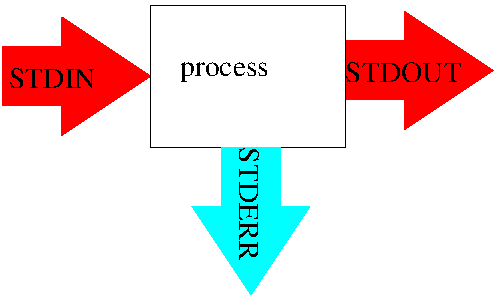
\includegraphics[width=1.2in]{../../slides/cmdline/process}
  \end{center}
  }
  \only<2>{
    \begin{center}
      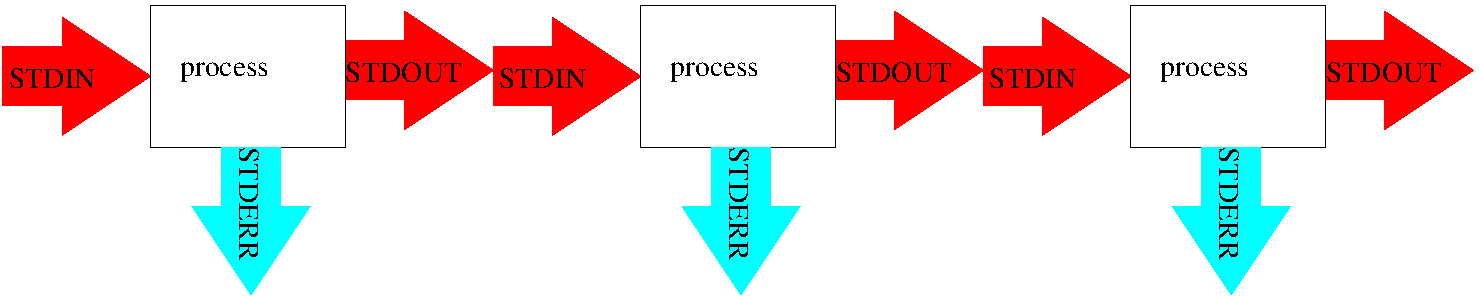
\includegraphics[width=3.6in]{../../slides/cmdline/processes}
    \end{center}
  }
  \begin{itemize}
    \item <1-> Каждое приложение открывает 3 стандартных файловых дескриптора stdin (fd 0), stdout(fd 1), stderr (fd 2)
    \item <2-> Приложения могут работать как фильтр из STDIN в STDOUT, можно объединять несколько приложений в конвейер
    \item <2-> Синтаксис {\tt <app1> | <app2>}
  \end{itemize}
\end{frame}
}

\section{Перенаправление ввода-вывода}
\mode<all>{

\begin{frame}{Конвееры}
%  \textbf{Цель} -- максимальная модульность: большое количество простых приложений, взаимодействующих друг с другом для решения задач
  \only<1>{
  \begin{center}
    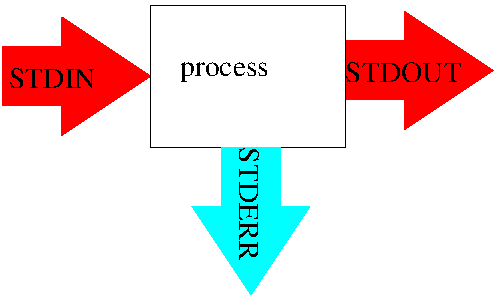
\includegraphics[width=1.2in]{../../slides/cmdline/process}
  \end{center}
  }
  \only<2>{
    \begin{center}
      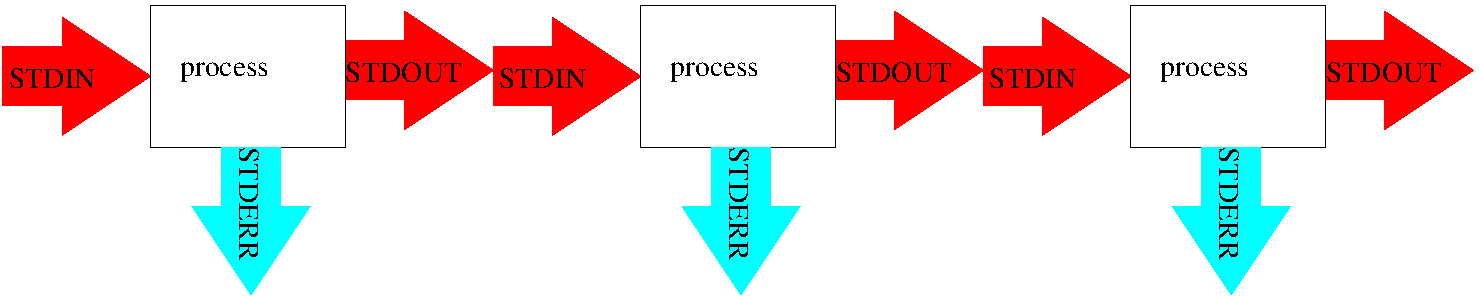
\includegraphics[width=3.6in]{../../slides/cmdline/processes}
    \end{center}
  }
  \begin{itemize}
    \item <1-> Каждое приложение открывает 3 стандартных файловых дескриптора stdin (fd 0), stdout(fd 1), stderr (fd 2)
    \item <2-> Приложения могут работать как фильтр из STDIN в STDOUT, можно объединять несколько приложений в конвейер
    \item <2-> Синтаксис {\tt <app1> | <app2>}
  \end{itemize}
\end{frame}
}
\mode<all>{\begin{frame}{Перенаправления в файл}

\begin{itemize}
  \item Перенаправление stdout 
    \begin{itemize}
      \item С созданием нового файла

        {\tt command > file}\\
		Например {\tt cat file1 file2 > file3}
      \item С дополнением существующего

		  {\tt command >\phantom{}>  file}
    \end{itemize}
    \pause
  \item Перенаправления stdin

    {\tt command < file}
    \pause
  \item Перенаправления stderr

    {\tt command1 2>\&1 | command2}

   {\tt command 1>file 2>\&1}

   {\tt command 2>file 1>\&2}
\end{itemize}

\end{frame}


}
\mode<all>{\begin{frame}[fragile]{Мультистрочный ввод (Here-документ)}

\begin{verbatim}
program <<LABEL
Тут
    много
	     строк
LABEL
\end{verbatim}

	\pause
	\begin{block}{Пример}
	Передадим несколько строк в COM-порт 1
\begin{lstlisting}[language=bash]
cat >/dev/ttyS0 <<E_O_F
ATZ
ATDT 8w0170123456
E_O_F
\end{lstlisting}
	\end{block}
\end{frame}
}

\part{Полезные команды}

\section{Полезные команды-1}

\mode<all>{\begin{frame}{Дополнительный набор команд}
  \begin{itemize}
    \item {\tt cat} - Вывод файла в stdout, соединение нескольких файлов в stdout
    \item {\tt wc} - подсчет статистики символов в файле или в stdin 
    \item {\tt sort} - сортировка строк файла
    \item {\tt uniq} - объединение одинаковых строк в одну
    \item {\tt tr} - замена набора символов
    \item {\tt less} - программа-пейджер
    \item {\tt grep} - поиск строк, соответствующих регулярному выражению
    \item {\tt cut} - выделение полей из строк stdin
    \item {\tt awk} - небольшой язык программирования (также полезен для выделения полей)
  \end{itemize}
\end{frame}

\begin{frame}[fragile]{Некоторые примеры использования}
\begin{lstlisting}[language=bash]
cat /proc/1/environ | tr '\0' '\n' | less
ls  | wc -l # подсчет числа файлов
man uniq | tr  '[:space:]' '\n' | sort | uniq -c | sort -n | less # подсчет количества слов в тексте man uniq
history | wc -l # подсчет ранее введенных команд
cat /etc/udev/rules.d/* | wc -l
ls -s *.jpg | awk 'BEGIN{s=0};/^[ ]*[0-9]/{s+=\$1};END{print s}' 
\end{lstlisting}
  \pause
  \begin{block}{Упражнение}
    Посчитать статистику использования команд в history
  \end{block}
\end{frame}

\begin{frame}{Дополнительный набор команд для работы с текстом}
	\begin{itemize}
	  \item {\tt head} -- вывести первые строки
	  \item {\tt tail} -- вывести последние строки
		\begin{itemize}
			\item {\tt -f} -- отслеживать добавление данных в файл 
		\end{itemize}
	  \item {\tt tee} -- копировать стандартный вывод в файл
	  \item {\tt grep} -- печать текста, соответствующего шаблону
		\begin{itemize}
			\item {\tt -i}	
			\item {\tt -v}
			\item {\tt -o}
		\end{itemize}
	\end{itemize}
\end{frame}

}

\subsection{Архиваторы}
\mode<all>{\begin{frame}[fragile]{Архивация}
	\begin{block}{Архивация: tar}
		\begin{itemize}
			\item {\tt -c} -- создать архив
			\item {\tt -x} -- извлечь из архива
				\begin{itemize}
					\item {\tt -C} -- перейти в директорию
					\item {\tt -{}-strip-components=N} -- пропустить N уровней
				\end{itemize}
			\item {\tt -f} -- запись в файл
		\end{itemize}
	\end{block}

	\begin{block}{Сжатие: gzip, bzip, xz}
		\begin{itemize}
			\item {\tt -[1-9]} -- изменить уровень сжатия
			\item {\tt -d} -- распаковать
			\item {\tt -c} -- вывод на консоль
		\end{itemize}
		\begin{verbatim}
dd if=/dev/sda bs=1M count=1 | gzip -c > backup.gz
		\end{verbatim}
	\end{block}

\end{frame}

\begin{frame}[fragile]{Архивация: примеры}

	Создать сжатый архив:
	\begin{verbatim}
tar -czf archive.tar.gz *
	\end{verbatim}
	\pause
	Распаковать сжатый архив в директорию {\tt /tmp}:
	\begin{verbatim}
tar -C /tmp/ -xzf archive.tar.gz 
	\end{verbatim}
	\pause
	Создать сжатый архив:
	\begin{verbatim}
tar -czf archive.tar.gz *
	\end{verbatim}
	\pause
	Создать копию текущей директории в директории {\tt /tmp/copy/}:
	\begin{verbatim}
tar -c * | tar -C /tmp/copy -x
tar -cf - * | tar -C /tmp -xf -
	\end{verbatim}
	\pause
	Создать копию текущей директории на другом хосте:
	\begin{verbatim}
HostDest: netcat -l 2222 | gzip -dc | tar -C /tmp/copy/ -x
HostSrc:  tar -c * | gzip -9 | netcat HostDest 2222
	\end{verbatim}
\end{frame}
}

\subsection{find и xargs}
\mode<all>{\begin{frame}[fragile]{Поиск файлов}
	\begin{block}{find}
		\begin{itemize}
			\item {\tt -type} -- тип файлового объекта
			\item {\tt -size} -- размер
			\item {\tt -maxdepth} -- глубина рекурсии
			\item {\tt -exec} -- выполнить команду
			\item {\tt -printf} -- форматированный вывод
		\end{itemize}
	\end{block}

	\begin{block}{Примеры}
		\begin{verbatim}
find /etc -type f -size +100k  -exec ls -l {} \;
		\end{verbatim}

		\begin{verbatim}
find -type d -user altlinux
		\end{verbatim}
	
	\end{block}
\end{frame}

\begin{frame}[fragile]{xargs}
	\begin{block}{xargs}
			Утилита для создания и запуска команд из стандартного потока ввода:
		\begin{verbatim}
xargs [options] command [command options]
		\end{verbatim}

		\begin{itemize}
			\item {\tt -d} -- разделитель
			\item {\tt -0} -- null-terminated строки
			\item {\tt -I text} -- подстановка
			\item {\tt -n N} -- максимальное количество аргументов
			\item {\tt -P N} -- максимальное количество процессов
		\end{itemize}

	\end{block}
\end{frame}

\begin{frame}[fragile]{xargs}
	\begin{block}{Примеры}
		\begin{verbatim}
find /etc -type f -size -100k | xargs tar -czf /tmp/archive-100k.tar.gz
		\end{verbatim}

		\begin{verbatim}
find /etc -type f | xargs -I {} echo "Найден {} файл"
		\end{verbatim}

		\begin{verbatim}
find . -type f -name "*.mp3" -print0 | xargs -0 -n 1 -P 0 -I mp3 avconv -i mp3 mp3.ogg
		\end{verbatim}
	
	\end{block}
\end{frame}


}

\subsection{Редакторы}
\mode<all>{\begin{frame}{Редакторы}
	\begin{itemize}
		\item Интерактивные
			\begin{itemize}
				\item vi
					\begin{itemize}
						\item Есть почти везде
					\end{itemize}
				\item vim
				\item emacs
			\end{itemize}
		\item Поточные
			\begin{itemize}
				\item {\tt ed}
				\item {\tt sed}
				\item {\tt awk}
			\end{itemize}
	\end{itemize}
\end{frame}

\begin{frame}[fragile]{Метасимволы}
	\begin{block}{grep, sed, awk}
	\end{block}
	\begin{itemize}
		\item {\tt .} -- любой символ за исключением пустой строки
		\item {\tt *} -- любоe количество символов, которые стоят перед {\tt *}
		\item {\tt \^{}} -- начало строки
		\item {\tt \$} -- конец строки
		\item {\tt [...]} -- любой символ из заключенных в скобки
	\end{itemize}
\end{frame}

\begin{frame}[fragile]{sed}
	\begin{block}{Сценарии}
		{\tt [ addr [ ,  addr ] ] cmd [ args ]}
	\end{block}

	\tiny
	\begin{block}{Команды}
		\begin{itemize}
		  \item {\tt a, i} -- добавить строку после (перед) текущей
			  \begin{verbatim} who | sed -e 'a Text' \end{verbatim}
		  \item {\tt c} -- удалить строку и заменить на текст
			  \begin{verbatim} who | sed -e "/$USER/ c Юзверь" \end{verbatim}
		  \item {\tt d} -- удалить строку
			  \begin{verbatim} who | sed -e '2,4 d' \end{verbatim}
			  \begin{verbatim} who | sed -e '/pts/ d' \end{verbatim}
		  \item {\tt s} -- замена по регулярному выражению
			  \begin{verbatim} who | sed -e "s/$USER/Юзверь/g" \end{verbatim}
		\end{itemize}
	\end{block}
\end{frame}


}

\part{Система управления пакетами}
\section{}
\mode<all>{\begin{frame}
	\frametitle{И еще раз про "DLL hell"}
	
	\begin{block}{Устанавливаем программу}
	А что же с библиотеками?
	\end{block}

	\pause

	\begin{columns}
		\column{0.5\textwidth}
		\begin{block}{"В системе все есть!"}
		\begin{itemize}
			\item Oh, really???
			\item И нужной версии?
			\item А API и ABI точно не менялись?
			\item А если библиотек несколько версий?
			\item А если нужны дополнительные программы?
		\end{itemize}
		\end{block}
		\pause
		\column{0.5\textwidth}
		\begin{block}{"Всё своё, ношу с собой!"}
		\begin{itemize}
			\item А как насчет объема?
			\item Использование памяти.
			\item А что насчет лицензий?
			\item И все-таки порядок загрузки...
			\item Не спасает от проблем с 3rd-party ПО.
		\end{itemize}
		\end{block}
	\end{columns}
\end{frame}

\begin{frame}
	\frametitle{Хаос}

	\begin{center}
		"Даешь каждой платформе и языку собственную систему управления пакетами!"
	\end{center}

	\begin{block}{Увы, мы не в идеальном мире}
		\begin{itemize}
			\item Дистрибутивы: rpm\{4,5\}, deb, portage, pacman... и куча модификаций...
			\item Дополнительный софт: {\tt ./configure; make; make install}
			\item Java: {\tt ivy, ant, maven, gradle}
			\item Ruby: gem
			\item Perl: CPAN
			\item Python: pip + PyPi
		\end{itemize}
	\end{block}

\end{frame}

\begin{frame}
	\frametitle{Разработка и использование в реальной системе}
	
	\begin{block}{Build-time vs Run-time}

		\begin{enumerate}
			\item Не все, что нужно во время компиляции, должно быть установлено в конечной системе.
			\item Не все, что нужно для работы программы, необходимо устанавливать на сборочной системе.
		\end{enumerate}
	\end{block}
%TODO перенести после описания структуры каталогов
	\begin{block}{Чистое сборочное окружение}
		\begin{itemize}
			\item Воспроизводимость сборки 
			\item Контроль зависимостей
			\item Контроль автоматически "подхваченных" зависимостей
		\end{itemize}
	\end{block}
\end{frame}

}

\mode<all>{\begin{frame}{Система управления пакетами: для чего это нужно}
\begin{itemize}
 \item ''DLL Hell''
 \item Dependency hell
 \item Общие задачи пакетного менеджера:
   \begin{itemize}
     \item Проверка целостности пакетов
     \item Проверка зависимостей пакетов
        \item Поддержание списка установленных пакетов
        \item Автоматическое удаление пакетов
     \item Предоставление доступа к репозиторию пакетов
     \item Разрешение зависимостей
   \end{itemize}
\end{itemize}
\end{frame}

\begin{frame}{Debian-based и RedHat-based системы управления пакетами}
\begin{center}
 \textbf{Два уровня пакетных менеджеров}
\end{center}
\begin{columns}
  \column{0.4\textwidth}
  \begin{center}
    \textbf{RedHat-based}
  \end{center}
  \begin{itemize}
    \item dnf/yum
    \item rpm
  \end{itemize}
  \column{0.4\textwidth}
  \begin{center}
    \textbf{Debian-based}
  \end{center}
  \begin{itemize}
    \item aptitude, apt, synaptic
    \item dpkg
  \end{itemize}
\end{columns}
\end{frame}
}

\mode<all>{\begin{frame}{RPM: команды}
	\begin{block}{Установка пакета}
		{\tt rpm -i [rpm-file1] ... [[url://]rpm-fileN] }
	\end{block}
	\begin{block}{Удаление пакета}
		{\tt rpm -e pkgname1 ... pkgnameN }
	\end{block}
	\begin{block}{Обновление пакета}
		{\tt rpm -U [rpm-file1] ... [[url://]rpm-fileN] }
	\end{block}
	\begin{block}{Проверка пакета}
		{\tt rpm -V pkgname1 ... pkgnameN }
	\end{block}
\end{frame}

\begin{frame}{RPM: часто используемые опции опроса}

	\begin{itemize}
		\item {\tt pkgname} -- выбор пакета, установленного в системе
		\item {\tt -a} -- все пакеты, установленные в системе
		\item {\tt -p} -- использовать файл RPM
	\end{itemize}


	\begin{itemize}
		\item {\tt -i} -- показать информацию пакета\\
			{\tt rpm -q -i glibc }
		\item {\tt -l} -- показать список файлов пакета \\
			{\tt rpm -q -l glibc }
		\item {\tt --whatprovides} -- \\
			{\tt rpm -q --whatprovides java}
		\item {\tt --whatrequires} -- \\
			{\tt rpm -q --whatrequires /bin/bash}
		\item {\tt --queryformat} -- формат вывода\\
			{\tt rpm -q --whatrequires /bin/bash --queryformat ''\%\{name\} ''}

	\end{itemize}

\end{frame}


}

\mode<all>{\newcounter{tmpc}

\begin{frame}{Репозиторий}
	\begin{block}{Репозиторий пакетов}
		Место, где хранятся и поддерживаются пакеты, а также сопутствующая мета-информация, предназначенное для использования пакетным менеджером.
	\end{block}
	\begin{block}{Пример: Fedora Core}
		\begin{itemize}
			\item Packages/*.rpm
			\item RPM-GPG-KEY-*
			\item repodata
			\begin{itemize}
				\item множество сжатых и несжатых XML файлов для YUM
			\end{itemize}
		\end{itemize}

		Описание репозтория для YUM на локальной системе хранится по пути
		{\tt /etc/yum.repos.d/*.repo}
	\end{block}
		
\end{frame}

\begin{frame}{YUM: команды}
	\begin{block}{Установка/обновление пакета}
		{\tt yum install pkgname }
	\end{block}
	\begin{block}{Обновление всех пакетов}
		{\tt yum update }
	\end{block}
	\begin{block}{Удаление пакета}
		{\tt yum remove pkgname }
	\end{block}
	\begin{block}{Поиск}
		{\tt yum list pkgname }\\
		{\tt yum search pkgname }
	\end{block}
\end{frame}


\begin{frame}[fragile]{Упражнение}
  \begin{enumerate}
      \item Создать на {\tt /dev/sda} раздел размером примерно 10Gb
      \item Создать на этом разделе ext3 ФС и смонтировать раздел в {\tt /mnt/chroot}
      \item Развернуть {\tt /media/nfs/pub/CentOS/precreated/centOS.tar.gz} в {\tt /mnt/chroot}
      \item Смонтировать {\tt proc, sysfs} а также {\tt /dev} в соответствующие места {\tt /mnt/chroot}
      \item {\tt chroot /mnt/chroot}
      \item Отредактировать {\tt /etc/resolv.conf} -- скопировать туда информацию из {\tt resolv.conf} основной системы
      \item Отредактировать {\tt /etc/yum.conf} Добавить следующий раздел
\begin{minipage}{0.5\textwidth}
\begin{verbatim}
[base]
  name = CentOS 6
  baseurl = ftp://192.168.11.15/CentOS
  gpgcheck = 0
\end{verbatim}
\end{minipage}
\setcounter{tmpc}{\theenumi}
\end{enumerate}
\end{frame}
\begin{frame}{Продолжение упражнения}
  \begin{enumerate}
      \setcounter{enumi}{\thetmpc}
      \item {\tt yum update}
      \item Установить пакет vim
      \item Посмотреть списки файлов для пакетов {\tt yum, rpm}
      \item Найти пакет предоставляющий сервис ssh и установить его
      \item Удалить пакет vim
    \end{enumerate}
\end{frame}


}

\part{Пользователи и привилегии}

\section{Многопользовательская модель UNIX}
\mode<all>{\begin{frame}{Многопользовательская модель}   
 \begin{itemize}
   \item Linux -- многопользовательская система
   \item Привилегии пользователей
     \begin{itemize}
       \item root
       \item other users
      \end{itemize}
     \end{itemize}
\end{frame}

\section{Механизмы разделения привилегий}
\subsection{Классический UNIX}

\begin{frame}{Пользователи, группы и файлы}
\begin{itemize}
  \item Каждый пользователь принадлежит одной или нескольким \textbf{группам}
  \item Каждый файл и директория принадлежит
    \begin{itemize}
      \item Одному пользователю 
      \item Одной группе
    \end{itemize}
  \pause
  \item  Разрешения что либо делать с файлом определяются по отношению к
    \begin{enumerate}
      \item Пользователю-владельцу файла
      \item Группе владеющей файлом
      \item Всем остальным пользователям
    \end{enumerate}

\end{itemize}
\pause
\begin{columns}
  \column{0.48\textwidth}
  \begin{itemize}
    \item {\tt ls -l} 3,4 поле 
    \item {\tt groups}
   \end{itemize}
  \column{0.48\textwidth}
  \begin{block}{Попробовать}
    {\tt ls -l /usr/bin/}

    {\tt groups}

    {\tt groups root}
  \end{block}
\end{columns}
\end{frame}


}

\mode<all>{\begin{frame}{Типы разрешений для файлов}
	\begin{columns}
		\column{0.48\textwidth}
		\begin{center}
			\textbf{Разрешения для файла}
		\end{center}
		\begin{itemize}
			\item Три типа разрешений
				\begin{enumerate}
					\item чтение read(r)
					\item запись write(w)
					\item выполнение execute(x)
				\end{enumerate}
		\end{itemize}
		\column{0.48\textwidth}
		\begin{center}
			\textbf{Разрешения для директорий}
		\end{center}
		\begin{itemize}
			\item Три типа разрешений
				\begin{enumerate}
					\item поиск файлов в директории read(r) 
					\item добавление и удаление файлов write(w)
					\item заход в директорию execute(x)
				\end{enumerate}
		\end{itemize}
	\end{columns}

	\pause

	Попробовать {\tt ls -l /usr/bin}

	\pause

	Пересчет мнемонического разрешения в битовую маску 

	$r\to4, w\to2 , x\to1$ 

	rwxrw-r-x$\to$765
\end{frame}

\begin{frame}{Команды для управления пользователями и разрешениями файлов}
	\begin{columns}
		\column{0.48\textwidth}
		\begin{itemize}
			\item {\tt chown}
			\item {\tt chmod}
		\end{itemize}
		\column{0.48\textwidth}
		\begin{itemize}
			\item {\tt useradd, usermod, userdel}
			\item {\tt groupadd, groupmod, groupdel}
			\item {\tt su, sudo}
		\end{itemize}
	\end{columns}
\end{frame}

\begin{frame}
	\begin{block}{Упражнения}
		\begin{enumerate}
			\item Создать директорию без r разрешения но с x разрешением, внутри нее создать поддиректорию с rwx разрешениями (для пользователя altlinux)
			\item Создать нового пользователя testuser.
			\item Скопировать {\tt /bin/bash} (под именем mysh) в домашнюю директорию пользователя altlinux  и поставить r-x разрешение только для other
			\item Попробовать выполнить скопированный файл от имени пользователя altlinux, затем от имени пользователя testuser
			\item Создать новую группу testgroup
			\item Изменить группу владеющую mysh на testgroup и сделать {\tt chmod 464 mysh}
			\item Попробовать выполнить mysh от имени altlinux и root. 
			\item Добавить пользователя altlinux в группу testgroup и попробовать выполнить mysh еще раз
			\item Получить список групп которым принадлежат устройства в {\tt /dev}
		\end{enumerate}
	\end{block}
\end{frame}

\begin{frame}{SUID программы}
	\begin{block}{Попробовать}
		{\tt id}

		{\tt ls -l `which su`}
	\end{block}
	\pause
	\begin{itemize}
		\item Некоторые программы должны выполняться от имени обычного пользователя, но иметь больше привилегий
		\item Для этого у них устанавливается suid или sgid биты
		\item Установка suid (например {\tt chmod 4710 <file>})
	\end{itemize}
	\pause
	\begin{block}{Упражнение}
		\begin{itemize}
			\item Под root создать копию утилиты {\tt id} (назвать, например, {\tt id2}) в директории /usr/bin/
			\item Установить suid бит для этой утилиты
			\item Запустить {\tt id2} от имени пользователя altlinux
			\item То же с sgid битом
		\end{itemize}
	\end{block}
\end{frame}

\begin{frame}{Опасности SUID}
	\begin{itemize}
		\item Возможность backdoor через suid программу
			\begin{itemize}
				\item Shell игнорирует effective uid
				\item Скрипты обычно тоже игнорируют
				\item nosuid mount option
			\end{itemize}
		\item Атака через buffer overflow в существующей suid программе
			\begin{itemize}
				\item не использовать strcpy, sprintf, ... в security critical
				\item А если все же не уследили
					\begin{itemize}
						\item рандомизация стека
						\item grsecurity
						\item частично selinux
					\end{itemize}
			\end{itemize}
	\end{itemize}
\end{frame}


\begin{frame}{SUID, SGID и sticky bit для директорий}
	\begin{itemize}
		\item sgid для директорий -- все поддиректории и файлы внутри имеют тот же group id
		\item suid -- игнорируется
		\item Зато есть sticky bit 
	\end{itemize}
\end{frame}

% End of 5-th lecture


}
\section{Внутренний механизм управления пользователями}
\mode<all>{\begin{frame}{Хранение информации о пользователях в системе}

	\begin{block}{\tt /etc/group}
		{\tt  group\_name:password:GID:user\_list}
	\end{block}
	
	\pause

	\begin{block}{\tt /etc/passwd}
		{\tt account:password:UID:GID:GECOS:directory:shell}

		\begin{itemize}
			\item {\tt *} -- пароль не задан
			\item {\tt x} -- пароль задан в файле {\tt /etc/shadows}
		\end{itemize}
	\end{block}

	\pause

	\begin{block}{\tt /etc/shadow}
		\begin{enumerate}
			\begin{columns}
			\column{0.3\textwidth}

			\item login name
			\item encrypted password
			\item date of last password change

			\column{0.3\textwidth}		
			\item minimum password age 
			\item maximum password age
			\item password warning period

			\column{0.3\textwidth}
			\item password inactivity period
			\item account expiration date
			\item reserved field

			\end{columns}
		\end{enumerate}
	\end{block}

\end{frame}

\begin{frame}{Практическое задание}
    \begin{itemize}
		\item Посмотреть права доступа к файлам {\tt group}, {\tt passwd}, {\tt shadow}\\
			{\tt ls -l /etc/{group, passwd, shadow}}
		\item Добавить пользователя и группу и посмотреть изменения в перечисленных файлах
		\item Cоздать пользователя без использования системных утилит (пароль взять такой же, как у существующего пользователя).
    \end{itemize}
	\pause
	 \begin{itemize}
		\item Изменить пароль пользователю с помощью утилиты {\tt passwd}%\\
%			Hint: {\tt /etc/passwdqc.conf}
		\item Сбросить пароль пользователю\\
			Hint: {\tt usermod}
    \end{itemize}
\end{frame}


}

\mode<all>{\begin{frame}{PAM}
	% http://www.opennet.ru/base/net/pam_linux.txt.html
	\begin{itemize}
		\item PAM это динамическая библиотека
		\item Конфигурация PAM
			\begin{itemize}
				\item {\tt /etc/pam.conf}
				\item {\tt /etc/pam.d/...}
					\begin{itemize}
						\item Сервисы
						\item system\_auth
					\end{itemize}
			\end{itemize}
	\end{itemize}

	\begin{block}{Формат записи}
		\begin{columns}
			\column{0.245\textwidth}
			\textbf{module type}
			 \begin{itemize}
				 \item auth
				 \item account
				 \item session
				 \item password
			 \end{itemize}
			 \column{0.245\textwidth}
			 \textbf{control flag}
			 \begin{itemize}
				 \item requisite
				 \item required
				 \item sufficient
				 \item optional
			 \end{itemize}
			 \column{0.245\textwidth}
			 \textbf{module name}
			 \column{0.245\textwidth}
			 \textbf{module options}
		 \end{columns}
	 \end{block}
\end{frame}

\begin{frame}{Диспетчер службы имен (NSS)}

	Важная информация для системы:
		
	\begin{itemize}
		\item Информация о пользователях (логин, группа, пароль и т.д.)
		\item Информация о сетевых ресурсах (имена хостов, протоколов, сервисов)
    \end{itemize}

	\pause

	\begin{block}{NSS}
		\begin{itemize}
			\item Конфигурация: {\tt /etc/nsswitch.conf}
			\item Динамические библиотеки сервисов: {\tt ls -1 /lib*/libnss\_*}
		\end{itemize}
	\end{block}

\end{frame}



}

\part{Сетевая подсистема}

\section{Основы работы с сетевой подсистемой}

\mode<all>{\begin{frame}{Сетевая подсистема Linux}

	\begin{block}{Cетевой интерфейс}

		Сетевой интерфейс в Linux -– это абстрактный именованный объект,  используемый для передачи 
		данных через некоторую линию связи без привязки к ее (линии связи) реализации.
	\end{block}
\end{frame}

\begin{frame}{Сетевая подсистема Linux}

	\center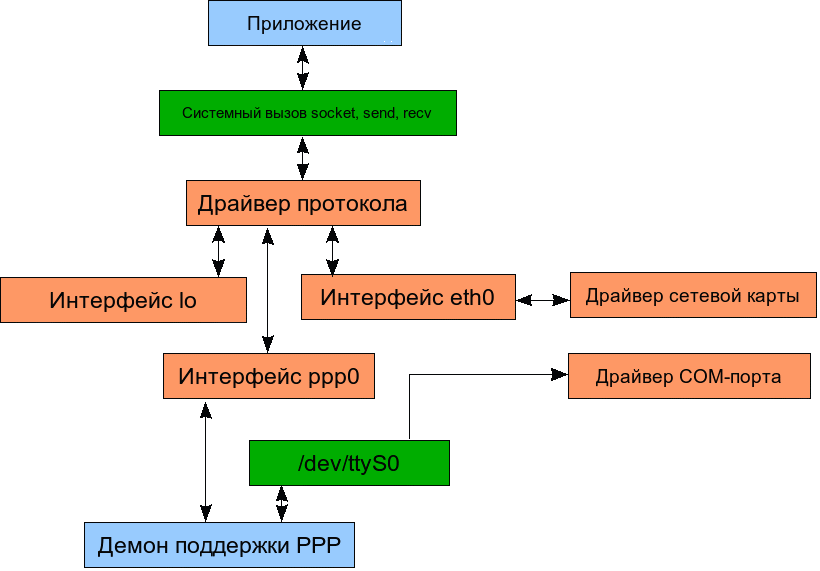
\includegraphics[height=0.8\textheight]{../../slides/networking/06-netstack.png}

\end{frame}


}

\subsection{Управление интерфейсами}
\mode<all>{\begin{frame}{Команды управления настройками сети}
	\begin{itemize}
	  \item ifconfig/route
	  \item iproute2
	\end{itemize}

	\begin{itemize}
		\item Список интерфейсов
			\begin{itemize}
				\item {\tt ifconfig -a}
				\item {\tt ip link show}
			\end{itemize}
		\item Включение интерфейса 
			\begin{itemize}
				\item {\tt ifconfig <iface> up}
				\item {\tt ip link set <iface> up}
			\end{itemize}
	  \item Выключение интерфейса
			\begin{itemize}
				\item {\tt ifconfig <iface> down}
				\item {\tt ip link set <iface> down}
			\end{itemize}
	  \item Назначение адреса
			\begin{itemize}
				\item {\tt ifconfig eth0 192.168.1.17 netmask 255.255.254.0 up}
				\item {\tt ip addr add 192.168.1.17/23 dev eth0}
			\end{itemize}
	\end{itemize}
\end{frame}

\begin{frame}{Конфигурационные файлы}
  \begin{itemize}
    \item {\tt /etc/resolv.conf}
    \item {\tt /etc/hosts}
	\item {\tt /etc/sysconfig/network}
    \item Расположение зависит от дистрибутива:
		\begin{itemize}
			\item RH-like: {\tt /etc/sysconfig/network-scripts}\\
				{\tt /etc/sysconfig/network-scripts/ifcfg-eth0}
			\item ALTLinux: {\tt /etc/net/ifaces}
			\item Debian: {\tt /etc/network/interfaces}
			\item Gentoo: {\tt /etc/conf.d/net}
		\end{itemize}
  \end{itemize}
\end{frame}

\begin{frame}{Дополнительные интерфейсы}
	\begin{block}{Алиасы}
		\begin{itemize}
			\item ifconfig <iface>:<alias> <ip> up
			\item ifconfig <iface> add <ip> up
			\item ip addr add <ip> {\bf label} <iface>:<alias> dev <iface>
		\end{itemize}
	\end{block}
	\pause
	\begin{block}{VLAN}
		\begin{itemize}
			\item vconfig add <iface> <id>
			\item vconfig rem <iface>{\bf.}<id>
			\item ip link add {\bf link} <iface> name <vlan\_name> {\bf type vlan id <id>}
			\item ip link delete <vlan\_name>
		\end{itemize}
	\end{block}

\end{frame}


}

\subsection{Полезные программы}
\mode<all>{\begin{frame}{Полезные утилиты}
	\begin{center}
		\begin{itemize}
			\item netstat / ss
			\item nslookup / dig
			\item ping
			\item traceroute
			\item tcpdump
			\item telnet
			\item netcat
			\item nmap
		\end{itemize}
	\end{center}

\end{frame}


\begin{frame}[allowframebreaks]{Полезные утилиты: практика}

		\begin{block}{netstat}

			Узнать:
			\begin{itemize}
				\item список используемых сокетов
				\item серверных сокетов
				\item имена/pid серверов
				\item узнать номера портов
			\end{itemize}
		\end{block}
	
		\framebreak
		\begin{block}{telnet/netcat}

			\begin{itemize}
				\item Чат по протоколу TCP с соседом
				\item Чат по протоколу UDP с соседом
				\item Передать текстовый и бинарный файлы
			\end{itemize}
	
			При создании чата использовать {\tt netstat} и {\tt tcpdump}
			для получения информации о соединении.
		\end{block}

		\framebreak
		\begin{block}{nmap}
			\begin{itemize}
				\item сканирование соседа
				\item сканирование выделенных портов у соседа (поиск сервера чата) 
				\item узнать список открытых портов на всех машинах в аудитории
				\item узнать список работающих машин
			\end{itemize}
		\end{block}
	
\end{frame}

tcpdump
0. pcap файлы/libpcap
1. запуск монитора
2. запуск чата
3. монитор-фильтр-анализ

}

\section{ssh}
\mode<all>{\begin{frame}{ssh}

	\begin{block}{ssh -- терминал}
		{\tt ssh [user@]host[:port]}\\
		{\tt ssh host [-l user] [-p port]}
		\begin{itemize}
			\item -v -- "разговорчивый" режим 
			\item -t -- насильное назначение псевдотерминала (для автоматизации)
		\end{itemize}
		Вся конфигурация пользователя: {\tt \$HOME/.ssh}
	\end{block}

	\pause

	\begin{block}{... и не только}
		\begin{itemize}
			\item -X -- "проброс" графики 
			\item -L [bindip:]port:rhost:rport -- "пробрасывание" порта с удаленной машины на локальную
			\item -R [bindip:]port:lhost:lport -- "пробрасывание" порта с локальной машины на удаленную
			\item -W host:port -- stdin/stdout с указанным хостом
			\item -D port -- динамический прокси
		\end{itemize}
	\end{block}
\end{frame}


}


\section{Дополнительные типы интерфейсов}

\subsection{alias, vlan}
\mode<all>{
\begin{frame}{Дополнительные интерфейсы}
	\begin{block}{Алиасы}
		\begin{itemize}
			\item ifconfig <iface>:<alias> <ip> up
			\item ifconfig <iface> add <ip> up
			\item ip addr add <ip> {\bf label} <iface>:<alias> dev <iface>
		\end{itemize}
	\end{block}
	\pause
	\begin{block}{VLAN}
		\begin{itemize}
			\item vconfig add <iface> <id>
			\item vconfig rem <iface>{\bf.}<id>
			\item ip link add {\bf link} <iface> name <vlan\_name> {\bf type vlan id <id>}
			\item ip link delete <vlan\_name>
		\end{itemize}
	\end{block}

\end{frame}


}
\subsection{Мосты}
\mode<all>{\begin{frame}{Мосты}
	\begin{itemize}
		\item Создать -- {\tt brctl addbr <bridge>}
		\item Удалить -- {\tt brctl delbr <bridge>}
		\item Добавить интерфейс -- {\tt brctl addif <bridge> <device>}
		\item Удалить интерфейс-- {\tt brctl addif <bridge> <device>}
	\end{itemize}
\end{frame}


}
\subsection{Тоннели}
\mode<all>{
\begin{frame}{''Виртуальные'' интерфейсы}
	\begin{block}{TUN/TAP}

		{\tt modprobe tun}

		\begin{itemize}
			\item Добавить интерфейс TUN -- {\tt tunctl -n -t <ifacename>}
			\item Добавить интерфейс TAP -- {\tt tunctl -p -t <ifacename>}
			\item Удалить интерфейс -- {\tt tunctl -d <ifacename>}
		\end{itemize}
	\end{block}

	\pause

	\begin{block}{Практика}
		\begin{itemize}
			\item Создать интерфейс TAP с именем {\tt mytap}
			\item Создать мост с именем {\tt mybr}
			\item Назначить интерфейсу {\tt mytap} адрес {\tt 192.168.0.<n>/24}
			\item Добавить интерфейсы {\tt mytap} и {\tt eth0} к мосту {\tt mybr}
			\item Запустить {\tt tcpdump} на интерфейсах {\tt mybr} и {\tt mytap}
			\item Запустить {\tt ping} соседа
		\end{itemize}
	\end{block}

\end{frame}


}

\section{Маршрутизация}
\mode<all>{\begin{frame}{Маршрутизация}
	\begin{itemize}
		\item netstat -r
		\item route
		\item ip route show
	\end{itemize}

	\begin{block}{Разрешить маршрутизацию на хосте}
		{\tt echo 1 > /proc/sys/net/ipv4/ip\_forward}
	\end{block}
\end{frame}


}

\section{iptables}
\mode<all>{\begin{frame}{Iptables}

	\center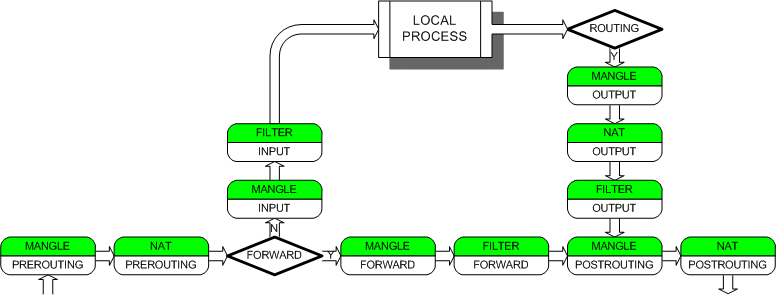
\includegraphics[height=0.4\textheight]{../../slides/networking/06-iptables.png}

	\begin{itemize}
	\begin{columns}
		\column{0.3\textwidth}
			\item[ ] {\bf iptables -L -t <table>}
				\bigskip

			\item filter -- файерволл
				\begin{itemize}
					\item INPUT
					\item FORWARD
					\item OUTPUT
				\end{itemize}
		\column{0.3\textwidth}
			\item nat -- преобразования адресов
				\begin{itemize}
					\item PREROUTING
					\item INPUT
					\item OUTPUT
					\item POSTROUTING
				\end{itemize}
		\column{0.3\textwidth}
			\item mangle -- специальные  изменения  пакетов (TOS, TTL, MARK)
				\begin{itemize}
					\item PREROUTING
					\item INPUT
					\item FORWARD
					\item OUTPUT
					\item POSTROUTING
				\end{itemize}
		\end{columns}
	\end{itemize}

\end{frame}


}

\part{Дисковая подсистема}

\section{Блочные устройства}
\mode<all>{\begin{frame}{Дисковая подсистема}

	\begin{block}{Блочное устройство}
		Вид файла устройств в UNIX/Linux-системах,  обеспечивающий интерфейс к устройству,
		реальному или виртуальному, в виде файла в файловой системе.
	\end{block}

	\begin{block}{Файловая система}
		Файловая система определяет формат содержимого и способ физического хранения информации,  
		которую принято группировать в виде файлов. 
		Конкретная файловая система определяет размер имени файла (директории),  
		максимальный возможный размер файла и раздела,  набор атрибутов файла.

		Распространенные для ОС Linux: ext2, ext4, xfs, reiserfs, vfat.
	\end{block}
\end{frame}

\begin{frame}{Примеры блочных устройств}

	\begin{itemize}
		\item {\tt /dev/{\bf s}d*}
		\item {\tt /dev/{\bf h}d*}
		\item {\tt /dev/ram*}
		\item {\tt /dev/loop*}
	\end{itemize}

	\begin{block}{Практическое задание:}
		\begin{enumerate}
			\item Посмотреть список вышеперечисленных устройств
			\item Посмотреть информацию об устройствах {\tt loop0, ram, sda}\\
				Hint: {\tt fdisk -l <device>}
		\end{enumerate}
	\end{block}
\end{frame}

\begin{frame}{Структура диска}
	\begin{columns}
		\column{0.6\textwidth}
		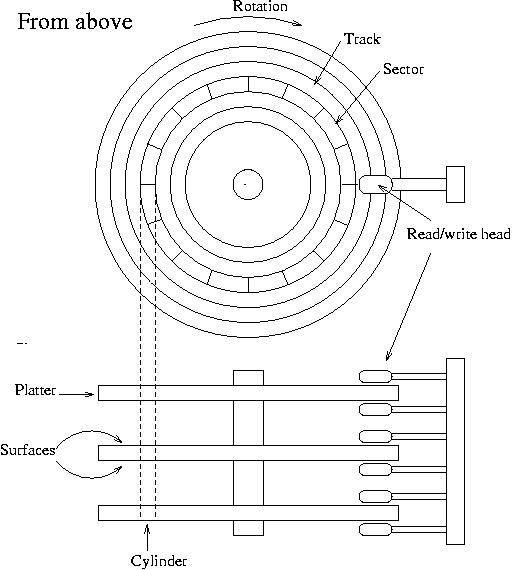
\includegraphics[height=0.8\textheight]{../../slides/disk/04-hd-schematic.png}
		\column{0.4\textwidth}
		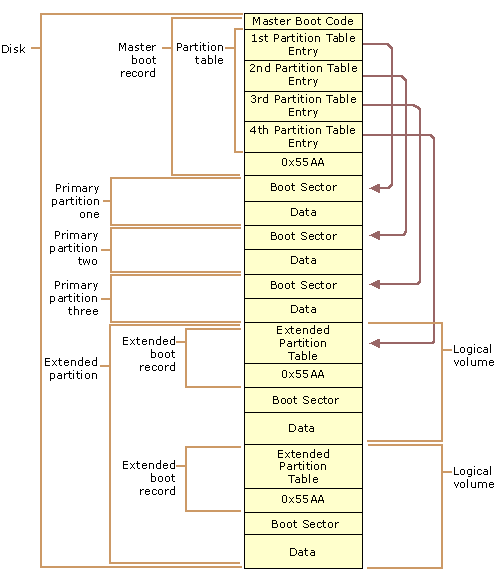
\includegraphics[height=0.8\textheight]{../../slides/disk/04-disk-structure.png}
	\end{columns}
\end{frame}

\begin{frame}{Отображение блочных устройств}


	\begin{block}{Device Mapper}
			{\tt /dev/mapper/*}\\
			device-mapper -- служит общим фреймворком для отображения одного блочного устройства на другое.

			Примеры: RAID, LVM, шифрованные диски и т.д.
	\end{block}

\end{frame}



}
\section{Основные команды}
\mode<all>{\begin{frame}{Полезные утилиты}
	\begin{columns}
		\column{0.25\textwidth}
		\begin{itemize}
			\item {\tt fdisk}
			\item {\tt parted}
			\item {\tt kpartx}
		\end{itemize}
		\column{0.25\textwidth}
		\begin{itemize}
			\item {\tt dd}
			\item {\tt losetup}
		\end{itemize}
		\column{0.25\textwidth}
		\begin{itemize}
			\item {\tt mkfs}
			\item {\tt fsck}
		\end{itemize}
		\column{0.25\textwidth}
		\begin{itemize}
			\item {\tt mount}
			\item {\tt umount}
			\item {\tt df}
		\end{itemize}
	\end{columns}

%	\bigskip
%	Понадобятся для упражнений:
%	\begin{itemize}
%			\item[*] {\tt chroot}
%			\item[*] {\tt kvm}
%	\end{itemize}
\end{frame}


\begin{frame}{Практика: отображение файла на loop-устройство}
	\begin{enumerate}
		\item Создать пустой файл размером 100MB: \\
			dd if=/dev/zero of=test bs=1M count=100
			\pause
		\item Найти неиспользуемое loop-устройство и отобразить на него файл:\\
			losetup -f \\
			losetup loop0 test
			\pause
		\item Посмотреть структуру loop-устройства, создать разделы и посмотреть результаты:\\
			fdisk -l /dev/loop0 \\
			fdisk /dev/loop0 \\
			fdisk -l /dev/loop0
			\pause
		\item Дать команду ядру перечитать разделы и создать устройства для разделов:\\
			ls -l /dev/mapper/* \\
			kpartx -a /dev/loop0 \\
			ls -l /dev/mapper/* \\
	\end{enumerate}
\end{frame}

\begin{frame}{Практика: создание файловой системы}
	\begin{enumerate}
		\item Форматируем файловую систему на устройстве: \\
			mkfs.ext2 /dev/mapper/loop0p1
			\pause
		\item и монтируем:\\
			mkdir -p /mnt/fs\\
			mount\\
			mount /dev/mapper/loop0p1 /mnt/fs\\
			mount\\
			df
			\pause
	\end{enumerate}
\end{frame}


\begin{frame}{Практика: чистимся}
	\begin{enumerate}
		\item Найти смонтированные разделы и отмонтировать их: \\
			mount \\
			umount /dev/mapper/loop0p1
			\pause
		\item Найти используемые loop-устройства\\
			losetup -a \\
			\pause
		\item Корректно удалить устройства для разделов:\\
			ls -l /dev/mapper/* \\
			kpartx -d /dev/loop0 \\
			ls -l /dev/mapper/* \\
			\pause
		\item Удалить отображение файла на loop-устройство: \\
			losetup -d /dev/loop0
	\end{enumerate}
\end{frame}


}
\section{GPT}
\mode<all>{\begin{frame}{GUID таблица разделов}

   \begin{columns}
      \column{0.5\textwidth}
      \begin{itemize}
        \item{Не менее 128 доступных разделов}
        \item{Дополнительные копии таблицы разделов}
        \item{$>1024^3$TB размер раздела}
        \item{Часть спецификации UEFI}
      \end{itemize}
      \column{0.5\textwidth}
      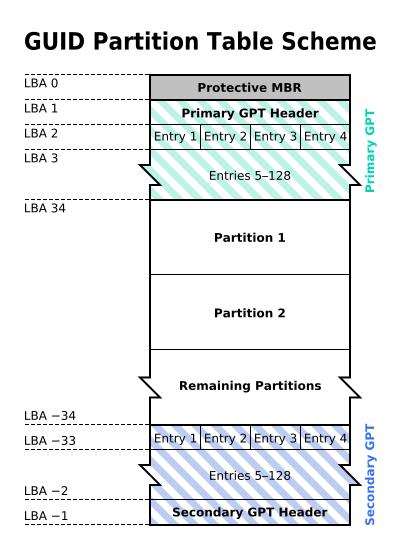
\includegraphics[width=0.9\textwidth]{../../slides/disk/gpt.png}
  \end{columns}
\end{frame}
\begin{frame}{Утилиты}
  \begin{itemize}
    \item gdisk (аналог fdisk)
    \item cgdisk (аналог cfdisk)
    \item parted
  \end{itemize}
\end{frame}

\begin{frame}{Источники по UEFI boot}
  \begin{itemize}
    \item http://www.rodsbooks.com/efi-bootloaders/
    \item http://www.slideshare.net/mlug/arch-onmac 
  \end{itemize}
\end{frame}
}
\section{LVM}
\mode<all>{\begin{frame}{LVM -- управление логическими томами}
  \begin{center}
    \textbf{Структура LVM}
  \end{center}
  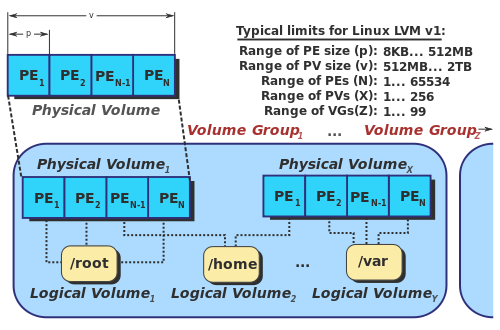
\includegraphics[width=0.7\textwidth]{../../slides/disk/LVM1-wiki.png}
\end{frame}

\begin{frame}{Преимущества LVM}
	\begin{itemize}
		\item Изменение размера
		\item Перемещение данных в активной системе
		\item Присвоение имен устройствам
		\item Чередование дисков
		\item Зеркалирование томов
		\item Снимки томов
	\end{itemize}
\end{frame}
 
\begin{frame}{LVM -- основные команды}
  \begin{itemize}
    \item Создание
      \begin{columns}
        \column{0.2\textwidth}
        \begin{itemize}
          \item pvcreate
        \end{itemize}
        \column{0.2\textwidth}
        \begin{itemize}
          \item vgcreate
        \end{itemize}
        \column{0.2\textwidth}
        \begin{itemize}
          \item lvcreate
        \end{itemize}
      \end{columns}
     \item Информация 
       \begin{columns}
         \column{0.2\textwidth}
         \begin{itemize}
           \item pvscan
           \item lvscan
           \item vgscan
		   \item lvmdiskscan
         \end{itemize}
         \column{0.2\textwidth}
         \begin{itemize}
           \item pvdisplay
           \item lvdisplay
           \item vgdisplay
		   \item[ ]
         \end{itemize}
         \column{0.2\textwidth}
         \begin{itemize}
           \item pvs
           \item lvs
           \item vgs
		   \item[ ]
         \end{itemize}
	 \end{columns}
      \item Манипулирование
        \begin{itemize}
          \item vgextend/vgreduce
          \item lvresize
          \item pvmove
          \item pvremove
         \end{itemize}
     \end{itemize}
    
\end{frame}

\begin{frame}{Упражнение: создание}
  \begin{enumerate}
    \item Создать 3 файла (200MB) и отобразить на {\tt /dev/loop[0-]}
	\item Найти устройства для работы с LVM {\tt lvmdiskscan}
	\item  {\tt pvcreate /dev/loop[0-2]}
    \item  {\tt pvscan, pvdisplay, pvs}
		\pause
    \item Создание группы томов {\tt vgcreate VG0 /dev/loop[0-2]}
    \item {\tt pvscan, vgscan, pvdisplay}
		\pause
    \item Создание логического тома {\tt lvcreate  -l 50\%VG -i 3 -n lv1 VG0}
	\item Создание файловой системы ext2 на {\tt /dev/VG0/lv1} и монтирование в {\tt /mnt/myfs}
	\end{enumerate}
\end{frame}


\begin{frame}{Упражнение: Создание снимка LVM}
  \begin{enumerate}
    \item Скопировать несколько файлов на { \tt /mnt/myfs}
    \item  {\tt lvcreate -\phantom{}-snapshot -l 10\%VG -n snap /dev/VG0/lv1}
    \item  {\tt lvdisplay, lvs, lvscan}
	\item Смонтировать снимок в {\tt /mnt/snap}
		\pause
    \item Удалить один из файлов на {\tt /mnt/snap/} или {\tt /mnt/myfs/}
	\item Отмонтировать снимок и оригинал
		\pause
	\item Объединяем снимок с оригиналом {\tt lvconvert -\phantom{}-merge VG0/snap}
	\item Монтируем {\tt /dev/VG0/lv1} в {\tt /mnt/myfs} и проверяем изменения
  \end{enumerate}
\end{frame}

\begin{frame}{Упражнение: изменение размера VG}
  \begin{enumerate}
%	\item Отмонтировать {\tt /mnt/myfs}
	\item Создать еще один файл и отобразить его на {\tt loop3}
	\item Увеличиваем размер группы {\tt vgextend VG0 /dev/loop3}
		\pause
    \item  {\tt pvscan; pvmove /dev/loop0; pvscan}
    \item  {\tt vgreduce VG0 /dev/loop0; pvscan}
    \item  {\tt pvremove /dev/loop0; pvscan}
  \end{enumerate}
\end{frame}


}


\end{document}
